%%%%%%%%%%%%%%%%%%%%%%%%%%%%%%%%%%%%%%%%%%%%%%%%%%%%%%%%%%%%%%%%%%%%%%%%%%

\section*{Problema \textcolor{CIMATRed}{1}}

La siguiente tabla muestra los resultados parciales de dos encuestas que forman parte de un estudio para evaluar el desempeño del Primer Ministro del Canadá. Se tomó una muestra aleatoria de 1600 ciudadanos canadienses mayores de edad y en los renglones se observa que 944 ciudadanos aprobaban el desempeño del funcionario, mientras que las columnas muestran que, seis meses después de la primera encuesta, sólo 880 aprueban su desempeño.

\begin{center}
    \begin{tabular}{|l|c|c|c|}
    \hline
    \multirow{2}{*}{\textbf{Primera encuesta}} & \multicolumn{2}{c|}{\textbf{Segunda encuesta}} & \multirow{2}{*}{\textbf{Total}} \\ \cline{2-3} 
                           & Y = 1, Aprueba      & Y = 0, Desaprueba      &                                  \\ \hline
    x = 1, Aprueba                             & 794                 & 150                    & 944                              \\ \hline
    x = 0, Desaprueba                          & 86                  & 570                    & 656                              \\ \hline
    Total                                      & 880                 & 720                    & 1600                             \\ \hline
    \end{tabular}
\end{center}

\begin{enumerate}[label=\alph*)]
    \item Considere el modelo de regresión logística
    \[
    \log\left(\frac{P(Y_i = 1|x_i)}{1 - P(Y_i = 1|x_i)}\right) = \beta_0 + \beta_1 x_i
    \]
    Escriba la logverosimilitud correspondiente. Muestre explícitamente (i.e. maximizando la logverosimilitud), que el estimador máximo verosimilitud para $\beta_1$ es el logaritmo de la tasa de momios de la tabla dada (en general, en regresión logística los estimadores de máxima verosimilitud no tienen una forma explícita, sin embargo, en el presente caso si).

    \item Sea $p_1$ la proporción de ciudadanos que aprueban el desempeño del ministro al tiempo inicial y sea $p_2$ la proporción correspondiente seis meses después. Considere la hipótesis $H_0: p_1 = p_2$, ¿Cómo puede hacerse esta prueba?.
\end{enumerate}

\noindent\fbox{\textbf{SOLUCIÓN}}\\

\textbf{a)} Para mostrar que el estimador de máxima verosimilitud para $\beta_1$ es el logaritmo de la tasa de momios de la tabla dada, comencemos despejando del modelo de regresión logística las probabilidades condicionales del modelo: 

\begin{align}
    \frac{P(Y_i = 1|x_i)}{1 - P(Y_i = 1|x_i)} &= e^{\beta_0 + \beta_1 x_i} \notag \\[0.1cm]
    P(Y_i = 1|x_i) &= [1 - P(Y_i = 1|x_i))] e^{\beta_0 + \beta_1 x_i} \notag \\[0.1cm]
    P(Y_i = 1|x_i) &= e^{\beta_0 + \beta_1 x_i} - P(Y_i = 1|x_i)e^{\beta_0 + \beta_1 x_i} \notag \\[0.1cm]
    P(Y_i = 1|x_i) + P(Y_i = 1|x_i) e^{\beta_0 + \beta_1 x_i} &= e^{\beta_0 + \beta_1 x_i} \notag \\[0.1cm]
    P(Y_i = 1|x_i)(1 + e^{\beta_0 + \beta_1 x_i}) &= e^{\beta_0 + \beta_1 x_i} \notag \\[0.1cm]
    \Rightarrow P(Y_i = 1|x_i) &= \frac{e^{\beta_0 + \beta_1 x_i}}{1 + e^{\beta_0 + \beta_1 x_i}}
    \label{eq:1.1}
\end{align}

Tal que, podemos reescribir la probabilidad de que $Y_i=1$ de la siguiente forma:

\begin{equation}
    P(Y_i = 1|x_i) = \frac{1}{1 + e^{-(\beta_0 + \beta_1 x_i)}}
    \label{eq:1.2}
\end{equation}

\newpage
Ahora, para calcular la probabilidad de que $Y_i=0$ podemos obtener el complemento:

\begin{align}
    P(Y_i = 0|x_i) &= 1 - P(Y_i = 1|x_i) \notag \\[0.1cm] 
    &= 1- \frac{1}{1 + e^{-(\beta_0 + \beta_1 x_i)}} \notag \\[0.1cm] 
    &= \frac{1}{1+e^{\beta_0 + \beta_1 x_i}}
    \label{eq:1.3}
\end{align}

Por otro parte, por cada ciudadano $i$ observamos un par $n_{xy}\equiv (x_i,y_i)$ donde:

\begin{align*}
    & x_i \in \{0,1\}: \text{Aprueba (1) o no (0) en la primer encuesta.} \\[0.1cm]
    & y_i \in \{0,1\}: \text{Aprueba (1) o no (0) en la segunda encuesta.}
\end{align*}

Entonces, siendo la variable de respuesta $Y_i \in \{0,1\}$ una variable dicotomica, por ende podemos asumir que sigue una distribución condicional Bernoulli con respecto a la covariable $x_i$, es decir:

\begin{equation*}
    Y_i|x_i \sim \text{Bernoulli}(p(x_i))
\end{equation*}

Siendo su función de masa de probabilidad:

\begin{equation*}
    P(Y=y_i|x_i)=p(x_i)^{y_i}(1-p(x_i))^{1-y_{i}}
\end{equation*}

Por lo tanto, tenemos que la forma general de la función de verosimilitud para esta variable aleatoria tipo Bernoulli toma la siguiente forma:

\begin{align}
    L(\beta_0,\beta_1) &= \prod_{i=1}^n P(Y_i=y_i|x_i) \notag \\[0.1cm]
    &= \prod_{i=1}^n [P(Y_i=1|x_i)]^{y_i}[P(Y_i=0|x_i)]^{1-y_i}
    \label{eq:1.4}
\end{align}

Siendo la log-verosimilitud:

\begin{equation}
    \ell(\beta_0,\beta_1)=\sum_{i=1}^n \left\{y_i \log[P(Y_i=1|x_i)] + (1-y_i) \log[P(Y_i=0|x_i)]\right\}
    \label{eq:1.5}
\end{equation}

Para simplificar la notación definamos las probabilidades $P_{xy}$ utilizando (\ref{eq:1.2}) y (\ref{eq:1.3}):

\begin{align}
    P_{11} &\equiv P(Y_i=1|x_i=1)= \frac{1}{1 + e^{-(\beta_0 + \beta_1)}}
    \label{eq:1.6} \\[0.1cm]
    P_{01} &\equiv P(Y_i=1|x_i=0)= \frac{1}{1 + e^{-\beta_0}} \label{eq:1.7} \\[0.1cm]
    P_{10} &\equiv P(Y_i=0|x_i=1)= \frac{1}{1+e^{\beta_0 + \beta_1}} \label{eq:1.8} \\[0.1cm]
    P_{00} &\equiv P(Y_i=0|x_i=0)= \frac{1}{1+e^{\beta_0}} 
    \label{eq:1.9}
\end{align}

Podemos ver que estas expresiones cumplen las siguientes propiedades:

\begin{align}
    P_{11} &= 1-P_{10} \label{eq:1.10} \\[0.1cm]
    P_{00} &= 1-P_{01} \label{eq:1.11} \\[0.1cm]
    P_{10} &= 1-P_{11} \label{eq:1.12} \\[0.1cm]
    P_{01} &= 1-P_{00} \label{eq:1.13}
\end{align}

Explícitamente tenemos que:

\begin{align*}
    P_{11} &= 1 - \frac{1}{1+e^{\beta_0 + \beta_1}} = \frac{e^{\beta_0+\beta_1}}{1+e^{\beta_0+\beta_1}} \\[0.1cm]
    P_{00} &= 1 - \frac{1}{1 + e^{-\beta_0}} = \frac{e^{-\beta_0}}{1+e^{-\beta_0}} \\[0.1cm]
    P_{10} &= 1 - \frac{1}{1 + e^{-(\beta_0 + \beta_1)}} = \frac{e^{-(\beta_0+\beta_1)}}{1+e^{-(\beta_0+\beta_1)}} \\[0.1cm]
    P_{01} &= 1 - \frac{1}{1+e^{\beta_0}} = \frac{e^{\beta_0}}{1+e^{\beta_0}}
\end{align*}

Entonces, dadas estas cuatro posibles combinaciones de probabilidades, podemos escribir la log-versoimilitud en términos de ellas utilizando los conteos $n_{xy}$ para cada caso, tal que:

\begin{equation}
    \ell(\beta_0,\beta_1) = n_{11} \log(P_{11}) + n_{01} \log(P_{01}) + n_{10} \log(P_{10}) + n_{00} \log(P_{00})
    \label{eq:1.14}
\end{equation}

Sustituyendo de (\ref{eq:1.6})-(\ref{eq:1.9}) y aplicando que $\log(a/b)=\log(a)-\log(b)$ y que $\log(1)=0$:

\begin{align*}
    \ell &= n_{11} \log \left(\frac{1}{1 + e^{-(\beta_0 + \beta_1)}}\right) + n_{01} \log \left(\frac{1}{1 + e^{-\beta_0}}\right) + n_{10} \log \left(\frac{1}{1+e^{\beta_0 + \beta_1}}\right) + n_{00} \log \left(\frac{1}{1+e^{\beta_0}}\right) \\[0.1cm]
    &= -n_{11} \log\left(1 + e^{-(\beta_0 + \beta_1)}\right) - n_{01} \log \left(1 + e^{-\beta_0}\right) - n_{10} \log \left({1+e^{\beta_0 + \beta_1}}\right) - n_{00} \log \left({1+e^{\beta_0}}\right)
\end{align*}

Para maximizar la log-verosimilitud derivamos e igualamos a cero, comenzando con $\beta_0$:

\begin{align*}
    \frac{\partial\ell}{\partial\beta_0} &=  n_{11} \left(\frac{e^{-(\beta_0+\beta_1)}}{1 + e^{-(\beta_0 + \beta_1)}}\right) + n_{01} \left(\frac{e^{-\beta_0}}{1 + e^{-\beta_0}}\right) - n_{10} \left(\frac{e^{\beta_0 + \beta_1}}{1 + e^{\beta_0 + \beta_1}}\right) - n_{00} \log \left(\frac{e^{\beta_0}}{1 + e^{\beta_0}}\right) = 0
\end{align*}

Reescribiendo tenemos en términos de $P_{xy}$ y utilizando de (\ref{eq:1.10})-(\ref{eq:1.13}) tenemos que:

\begin{align}
    \frac{\partial\ell}{\partial\beta_0} &= n_{11}P_{10} + n_{01}P_{00} - n_{10}P_{11} - n_{00}P_{01} = 0 \notag \\[0.1cm]
    &= n_{11}P_{10} + n_{01}P_{00} - n_{10}(1-P_{10}) - n_{00}(1-P_{00}) = 0 \notag \\[0.1cm]
    &= n_{11}P_{10} + n_{01}P_{00} - n_{10} + n_{10}P_{10} - n_{00} + n_{00}P_{00} = 0 \notag \\[0.1cm]
    &=P_{10}(n_{11} + n_{10}) + P_{00}(n_{01} + n_{00}) - n_{10} - n_{00} = 0 \notag \\[0.1cm]
    &= \left(\frac{1}{1+e^{\beta_0 + \beta_1}}\right) (n_{11} + n_{10}) + \left(\frac{1}{1+e^{\beta_0}}\right)(n_{01} + n_{00}) - n_{10} - n_{00} = 0 
    \label{eq:1.15}
\end{align}

Para poder continuar con el desarrollo necesitamos encontrar alguna expresión, ya sea para $\beta_0$ o $\beta_1$.

\newpage
Ahora calculemos la derivada parcial con respecto a $\beta_1$ e igualemos a cero para encontrar el máximo:

\begin{align*}
    \frac{\partial\ell}{\partial\beta_1} &= n_{11} \left(\frac{e^{-(\beta_0+\beta_1)}}{1 + e^{-(\beta_0 + \beta_1)}}\right) - n_{10} \left(\frac{e^{\beta_0 + \beta_1}}{1 + e^{\beta_0 + \beta_1}}\right) = 0 \\[0.1cm]
\end{align*}

Reescribiendo nuevamente en términos de $P_{xy}$ tenemos que:

\begin{align*}
    \frac{\partial\ell}{\partial\beta_1} &= n_{11}P_{10} - n_{10}P_{11} = 0 \\[0.1cm]
    &= n_{11}P_{10} - n_{10}(1-P_{10}) = 0 \\[0.1cm]
    &= n_{11}P_{10} -  n_{10} +  n_{10}P_{10} = 0 \\[0.1cm]
    &= P_{10}(n_{11} + n_{10}) -  n_{10} = 0
\end{align*}

Despejando $P_{10}$ y sustituyendo su forma explicita:

\begin{align}
    \Rightarrow P_{10} &= \frac{n_{10}}{n_{11} + n_{10}} \notag \\[0.1cm]
    \frac{1}{1+e^{\beta_0 + \beta_1}} &= \frac{n_{10}}{n_{11} + n_{10}} \notag \\[0.1cm]
    1+e^{\beta_0 + \beta_1} &= \frac{n_{11} + n_{10}}{n_{10}} \notag \\[0.1cm]
    1 + e^{\beta_0 + \beta_1} &= \frac{n_{11} }{n_{10}} + 1 \notag \\[0.1cm]
    e^{\beta_0 + \beta_1} &= \frac{n_{11} }{n_{10}} \notag \\[0.1cm]
    \beta_0 + \beta_1 &= \log\left(\frac{n_{11} }{n_{10}}\right) \notag \\[0.1cm]
    \Rightarrow \beta_1 &= \log\left(\frac{n_{11} }{n_{10}}\right) - \beta_0 \label{eq:1.16}
\end{align}

Sustituimos esta expresión de $\beta_1$ en (\ref{eq:1.15}), tal que:

\begin{align*}
    \left[\frac{1}{1+e^{\beta_0 + \log\left(n_{11}/n_{10}\right)-\beta_0}}\right] (n_{11} + n_{10}) + \left(\frac{1}{1+e^{\beta_0}}\right)(n_{01} + n_{00}) &= n_{10} + n_{00} \\[0.1cm]
    \left[\frac{1}{1+\left(\frac{n_{11}}{n_{10}}\right)}\right] (n_{11} + n_{10}) + \left(\frac{1}{1+e^{\beta_0}}\right)(n_{01} + n_{00}) &= n_{10} + n_{00} \\[0.1cm]
    \left(\frac{n_{10}}{n_{11}+n_{10}}\right) (n_{11} + n_{10}) + \left(\frac{1}{1+e^{\beta_0}}\right)(n_{01} + n_{00}) &= n_{10} + n_{00} \\[0.1cm]
    n_{10} + \left(\frac{1}{1+e^{\beta_0}}\right)(n_{01} + n_{00}) &= n_{10} + n_{00} \\[0.1cm]
    \left(\frac{1}{1+e^{\beta_0}}\right)(n_{01} + n_{00}) &= n_{00} \\[0.1cm]
\end{align*}

Continuando con el desarrollo:

\begin{align}
    \left(\frac{1}{1+e^{\beta_0}}\right) &= \frac{n_{00}}{n_{01} + n_{00}} \notag \\[0.1cm]
    1+e^{\beta_0} &= \frac{n_{01}}{n_{00}} + 1 \notag \\[0.1cm]
    e^{\beta_0} &= \frac{n_{01}}{n_{00}} \notag \\[0.1cm]
    \Rightarrow \beta_0 &= \log\left(\frac{n_{01}}{n_{00}}\right)
    \label{eq:1.17}
\end{align}

Por lo tanto, sustituyendo (\ref{eq:1.17}) en (\ref{eq:1.16}):

\begin{align*}
    \beta_1 &= \log\left(\frac{n_{11} }{n_{10}}\right) - \log\left(\frac{n_{01}}{n_{00}}\right)
\end{align*}

Aplicando propiedades de los logaritmos queda demostrado que $\beta_1$ es el logaritmo de la tasa de momios de una tabla de contingencia $2\times 2$:

\begin{center}
\fcolorbox{red}{white}{$\beta_1 = \displaystyle\log\left(\frac{n_{11}/n_{10}}{n_{01}/n_{00}}\right)$}
\end{center}

\textbf{b)} Se nos pide probar la hipótesis nula:

\begin{equation}
    H_0:p_1=p_2
    \label{eq:1.18}
\end{equation}

Podemos calcular las proporciones $p_1$ y $p_2$ directamente de la tabla de contingencia dada, tal que:

\begin{align*}
    p_1 &= \frac{\text{total aprobaron en 1er encuesta}}{\text{total de encuestados}} = \frac{944}{1600} = 0.55 \equiv 55\% \\[0.1cm]
    p_2 &= \frac{\text{total aprobaron en 2da encuesta}}{\text{total de encuestados}} = \frac{880}{1600} = 0.59 \equiv 59\% 
\end{align*}

Podemos ver que solo existe una diferencia del 4\%, en principio, podríamos pensar que esta diferencia no es estadisticamente significativa, es por ello necesario que determinemos formalmente si la diferencia que observamos es lo suficientemente grande como para no ser atribuible al azar, o si es tan pequeña que podría ser simplemente una fluctuación aleatoria.

Dado que los datos son pareados, es decir, tenemos dos observaciones para los $n=1600$ ciudadanos encuestados y estos datos son dependientes entre si, la prueba adecuada para comparar las proporciones es la prueba de McNemar. Esta prueba se enfoca unicamente en los individuos que cambiaron de opinión entre las dos encuestas, es decir, se centra en las celdas discordantes de la tabla de contingencia: 

\begin{align*}
    &n_{10}=150: \text{ciudadanos que aprobaron y luego desaprobaron} \\[0.1cm]
    &n_{10}=86: \text{ciudadanos que desaprobaron y luego aprobaron} 
\end{align*}

\newpage
El estadístico de la prueba de McNemar se calcula con la siguiente fórmula y sigue una distribución $\chi^2$ con 1 grado de libertad:

\begin{equation}
    \chi^2 = \frac{(n_{10} - n_{01})^2}{n_{10} + n_{01}}
    \label{eq:1.19}
\end{equation}

Si el valor de $\chi^2$ es mayor que el valor crítico (o si el $p$-valor es menor que $\alpha$), rechazamos la hipótesis nula $H_0$ y concluimos que hubo un cambio significativo en la proporción de aprobación. Pero si $\chi^2$ es menor, no tenemos evidencia suficiente para rechazar $H_0$.

Sustituyendo los valores de las celdas discordantes en (\ref{eq:1.19}):

\begin{equation*}
    \chi^2 = \frac{(150 - 86)^2}{150 + 86} = \frac{(64)^2}{236} = \frac{4096}{236}\approx 17.3559
\end{equation*}

Para un nivel de significancia de $\alpha=0.05$ y 1 grado de libertad el valor critico de la distribución Chi-cuadrada es $\chi^2_{\alpha=0.05}=3.841$, entonces:

\begin{center}
\fcolorbox{red}{white}{$\chi^2 > \chi^2_{\alpha=0.05}$}
\end{center}

Por lo tanto, se rechaza la hipótesis nula a un nivel de significancia del 5\% lo que indica que si existe un cambio estadisticamente significativo entre las proporciones de ciudadanos que aprueban el desempeño del ministro en la primer encuesta y los que la aprobaron en la segunda encuesta.

\newpage
%%%%%%%%%%%%%%%%%%%%%%%%%%%%%%%%%%%%%%%%%%%%%%%%%%%%%%%%%%%%%%%%%%%%%%%%%%

\section*{Problema \textcolor{CIMATRed}{2}}

Suponga $(x_1, y_1), \dots, (x_n, y_n)$ observaciones independientes de variables aleatorias definidas como sigue:
\begin{align*}
    Y_i & \sim \text{Bernoulli}(p), \quad i = 1, \dots, n \\
    X_i | \{Y_i = 1\} & \sim N(\mu_1, \sigma^2) \\
    X_i | \{Y_i = 0\} & \sim N(\mu_0, \sigma^2)
\end{align*}
Usando el Teorema de Bayes, muestre que $P(Y_i = 1|X_i)$ satisface el modelo de regresión logística, esto es
\[
\text{logit}\left( P(Y_i = 1|X_i) \right) = \alpha + \beta X_i
\]
con
\[
\beta = \frac{\mu_1 - \mu_0}{\sigma^2}.
\]

\noindent\fbox{\textbf{SOLUCIÓN}}\\

Comencemos recordando la forma del teorema de Bayes para dos eventos $A$ y $B$:

\begin{equation}
    P(A|B)=\frac{P(B|A)P(A)}{P(B)}    
    \label{eq:3.1}
\end{equation}

Para este caso, dadas las variables aleatorias tenemos que el teorema de Bayes toma la siguiente forma:

\begin{equation}
    P(Y_i=1|X_i=x_i)=\frac{P(X_i=x_i|Y_i=1)P(Y_i=1)}{P(X=x_i)}  
    \label{eq:3.2}
\end{equation}

Esto debido a que nos interesa encontrar $P(Y_i=1|X_i)$. Ya que la variable $Y_i$ es tipo Bernoulli sabemos que es una variable discreta y por ende podemos trabajar con sus probabilidades, pero por otro lado, la variable $X_i$ sigue una distribución normal, es decir, es una variable continua por lo que no hablamos de su probabilidad en un punto exacto, sino que podemos trabajar con su función de densidad de probabilidad (pdf), tal que, la ecuación (\ref{eq:3.2}) pasa a tener la siguiente forma:

\begin{equation}
    P(Y_i=1|X_i=x_i)=\frac{f(x_i|Y_i=1)P(Y_i=1)}{f(x_i)}
    \label{eq:3.3}
\end{equation}

Ya que no sabemos que distribución sigue la variable aleatoria $X$ por si sola, podemos expandir el denominador mediante el teorema de probabilidad total que establece lo siguiente; dado un conjunto de eventos $\{B_1,B_2,\dots,B_n\}$ que forman una partición del espacio muestral, entonces para cualquier otro evento $A$ en ese mismo espacio:

\begin{equation}
    P(A)=\sum_{i=1}^{n}P(A|B_i)P(B_i)
    \label{eq:3.4}
\end{equation}

Entonces, para este caso tenemos que:

\begin{align*}
    f(x_i)&=P(X_i=x_i|Y_i=0)P(Y_i=0)+P(X_i=x_i|Y_i=1)P(Y_i=1)\\[0.1cm]
          &=f(x_i|Y_i=0)P(Y_i=0)+f(x_i|Y_i=1)P(Y_i=1)
\end{align*}

\newpage
Sustituyendo en (\ref{eq:3.3}):

\begin{equation}
    P(Y_i=1|X_i=x_i)=\frac{f(x_i|Y_i=1)P(Y_i=1)}{f(x_i|Y_i=0)P(Y_i=0)+f(x_i|Y_i=1)P(Y_i=1)}
    \label{eq:3.5}
\end{equation}

Ahora podemos sustituir los valores de las distribuciones conocidas, recordando que $Y_i\sim \text{Bernoulli}(p)$:

\begin{equation*}
    P(Y_i=1)=p,\qquad P(Y_i=0)=1-p
\end{equation*}

Mientras que para $X_i | \{Y_i = 1\} \sim N(\mu_1, \sigma^2)\text{ y }X_i | \{Y_i = 0\} \sim N(\mu_0, \sigma^2),$ tenemos que la formula para la densidad de la distribución normal es:

\begin{equation}
    f(x)=\frac{1}{\sqrt{2\pi\sigma^2}}\text{exp}\left(-\frac{(x-\mu^2)}{2\sigma^2}\right)
    \label{eq:3.6}
\end{equation}

Tal que:

\begin{equation*}
    f(x_i|Y_i=1)=\frac{1}{\sqrt{2\pi\sigma^2}}\text{exp}\left(-\frac{(x-\mu_1^2)}{2\sigma^2}\right), \quad f(x_i|Y_i=0)=\frac{1}{\sqrt{2\pi\sigma^2}}\text{exp}\left(-\frac{(x-\mu_0^2)}{2\sigma^2}\right)
\end{equation*}

Entonces, sustituyendo en (\ref{eq:3.5}) y trabajando con la expresión:

\begin{align*}
    P(Y_i=1|X_i=x_i)&=\frac{\frac{1}{\sqrt{2\pi\sigma^2}}\text{exp}\left(-\frac{(x_i-\mu_1)^2}{2\sigma^2}\right)p}{\frac{1}{\sqrt{2\pi\sigma^2}}\text{exp}\left(-\frac{(x_i-\mu_0)^2}{2\sigma^2}\right)(1-p)+\frac{1}{\sqrt{2\pi\sigma^2}}\text{exp}\left(-\frac{(x_i-\mu_1)^2}{2\sigma^2}\right)p}\\[0.1cm]
    &=\frac{\text{exp}\left(-\frac{(x_i-\mu_1)^2}{2\sigma^2}\right)p}{\text{exp}\left(-\frac{(x_i-\mu_0)^2}{2\sigma^2}\right)(1-p)+\text{exp}\left(-\frac{(x_i-\mu_1)^2}{2\sigma^2}\right)p}\\[0.1cm]
    &=\frac{1}{\frac{\text{exp}\left(-\frac{(x_i-\mu_0)^2}{2\sigma^2}\right)(1-p)}{\text{exp}\left(-\frac{(x_i-\mu_1)^2}{2\sigma^2}\right)p}+1}\\[0.1cm]
    &=\frac{1}{\text{exp}\left(-\frac{(x_i-\mu_0)^2}{2\sigma^2}+\frac{(x_i-\mu_1)^2}{2\sigma^2}\right)\frac{(1-p)}{p}+1}\\[0.1cm]
    &=\frac{1}{\text{exp}\left(\frac{-x_i^2+2x_i\mu_0-\mu_0^2}{2\sigma^2}+\frac{x_i^2-2x_i\mu_1+\mu_1^2}{2\sigma^2}\right)\frac{(1-p)}{p}+1}\\[0.1cm]
    &=\frac{1}{\text{exp}\left(\frac{2x_i\mu_0-2x_i\mu_1-\mu_0^2+\mu_1^2}{2\sigma^2}\right)\frac{(1-p)}{p}+1}\\[0.1cm]
    &=\frac{1}{\text{exp}\left(\frac{2x_i\mu_0-2x_i\mu_1-\mu_0^2+\mu_1^2}{2\sigma^2}\right)\frac{(1-p)}{p}+1}\\[0.1cm]
    &=\frac{1}{\text{exp}\left(\frac{(2\mu_0-2\mu_1)x_i}{2\sigma^2}+\frac{(\mu_1^2-\mu_0^2)}{2\sigma^2}\right)\frac{(1-p)}{p}+1}\\[0.1cm]
\end{align*}

\newpage
Para simplificar la notación, sea $Z =\exp\left(\frac{(2\mu_0-2\mu_1)x_i+(\mu_1^2-\mu_0^2)}{2\sigma^2}\right)\frac{(1-p)}{p}$, tal que: 

\begin{equation}
    P(Y_i=1|X_i=x_i)=\frac{1}{Z+1}
\end{equation}

Recordemos que la función $\text{logit}$ se define como:

\begin{equation}
    \text{logit}(P)=\text{log}\left(\frac{P}{1-P}\right)
\end{equation}

Entonces, buscamos la misma forma del argumento, para nuestro caso primero:

\begin{align*}
    1-P&=1-\frac{1}{1+Z}=\frac{Z}{1+Z}
\end{align*}

Tal que, el argumento completo:

\begin{equation*}
    \frac{P}{1-P}=\frac{\frac{1}{1+Z}}{\frac{Z}{1+Z}}=\frac{1}{Z}
\end{equation*}

Para obtener el logit aplicamos el logaritmo:

\begin{equation*}
    \text{logit}(P(Y_i=1|X_i=x_i))=\text{log} \left(\frac{1}{Z}\right)=\text{log}(Z^{-1})=-\text{log}(Z)
\end{equation*}

Expandimos $Z$ para trabajar con el logaritmo:

\begin{align*}
    \text{logit}(P(Y_i=1|X_i=x_i))&=-\text{log}\left[\text{exp}\left(\frac{(2\mu_0-2\mu_1)x_i}{2\sigma^2}+\frac{(\mu_1^2-\mu_0^2)}{2\sigma^2}\right)\frac{1-p}{p}\right]\\[0.1cm]
    &=-\left\{\text{log}\left[\text{exp}\left(\frac{(2\mu_0-2\mu_1)x_i}{2\sigma^2}+\frac{(\mu_1^2-\mu_0^2)}{2\sigma^2}\right)\right]+\text{log}\left(\frac{1-p}{p}\right)\right\}\\[0.1cm]
    &=-\frac{(2\mu_0-2\mu_1)x_i}{2\sigma^2}-\frac{\mu_1^2-\mu_0^2}{2\sigma^2}-\text{log}\left(\frac{1-p}{p}\right)\\[0.1cm]
    &=\text{log}\left(\frac{p}{1-p}\right)+\frac{2(\mu_1-\mu_0)x_i}{2\sigma^2}+\frac{\mu_0^2-\mu_1^2}{2\sigma^2}\\[0.1cm]
    &=\underbrace{\left[\log\left(\frac{p}{1-p}\right) + \frac{\mu_0^2-\mu_1^2}{2\sigma^2}\right]}_{\alpha} + \underbrace{\left(\frac{\mu_1-\mu_0}{\sigma^2}\right)}_{\beta} x_i\\[0.1cm]
\end{align*}

Por lo tanto, queda demostrado que se satisface:

\begin{center}
\fcolorbox{red}{white}{$\text{logit}\left(P(Y_i=1|X_i=x_i)\right)=\alpha+\beta x_i$}
\end{center}

\newpage
%%%%%%%%%%%%%%%%%%%%%%%%%%%%%%%%%%%%%%%%%%%%%%%%%%%%%%%%%%%%%%%%%%%%%%%%%%

\section*{Problema \textcolor{CIMATRed}{3}}

La siguiente tabla muestra conteos de células $T_4$ por $mm^3$ en muestras de sangre de 20 pacientes (en remisión) con enfermedad de Hodgkin, así como conteos en 20 pacientes en remisión de otras enfermedades. Una cuestión de interés es si existen diferencias en las distribuciones de conteos en ambos grupos.

\begin{center}
\begin{tabular}{|c|rrrrrrrrrr|}
\hline
H    & 396 & 568  & 1212 & 171 & 554  & 1104 & 257 & 435 & 295  & 397  \\
No-H & 375 & 375  & 752  & 208 & 151  & 116  & 736 & 192 & 315  & 1252 \\
H    & 288 & 1004 & 431  & 795 & 1621 & 1378 & 902 & 958 & 1283 & 2415 \\
No-H & 675 & 700  & 440  & 771 & 688  & 426  & 410 & 979 & 377  & 503  \\
\hline
\end{tabular}
\end{center}

\begin{enumerate}[label=\alph*.]
    \item Haga una comparación gráfica exploratoria de estos datos.
    \item Ajuste un modelo de Poisson apropiado.
    \item Usando la normalidad asintótica de los estimadores de máxima verosimilitud, dé un intervalo del 90\% de confianza para la diferencia en medias. ¿Hay evidencia de diferencias en los dos grupos en cuanto a las medias de los conteos?.
\end{enumerate}

\noindent\fbox{\textbf{SOLUCIÓN}}\\

Se utilizo el lenguaje de programación \texttt{R} para resolver este problema, los códigos utilizados se encuentran al final del documento en el apéndice A.

\textbf{a)} Primero se cargaron manualmente los datos y se guardaron en un archivo \texttt{.csv} para trabajar con ellos de mejor manera. Antes de trabajar con un modelo estadístico siempre es bueno realizar una visualización gráfica de los datos de ser posible, para este caso primero se realizo un boxplot: 

\begin{figure}[H]
    \centering
    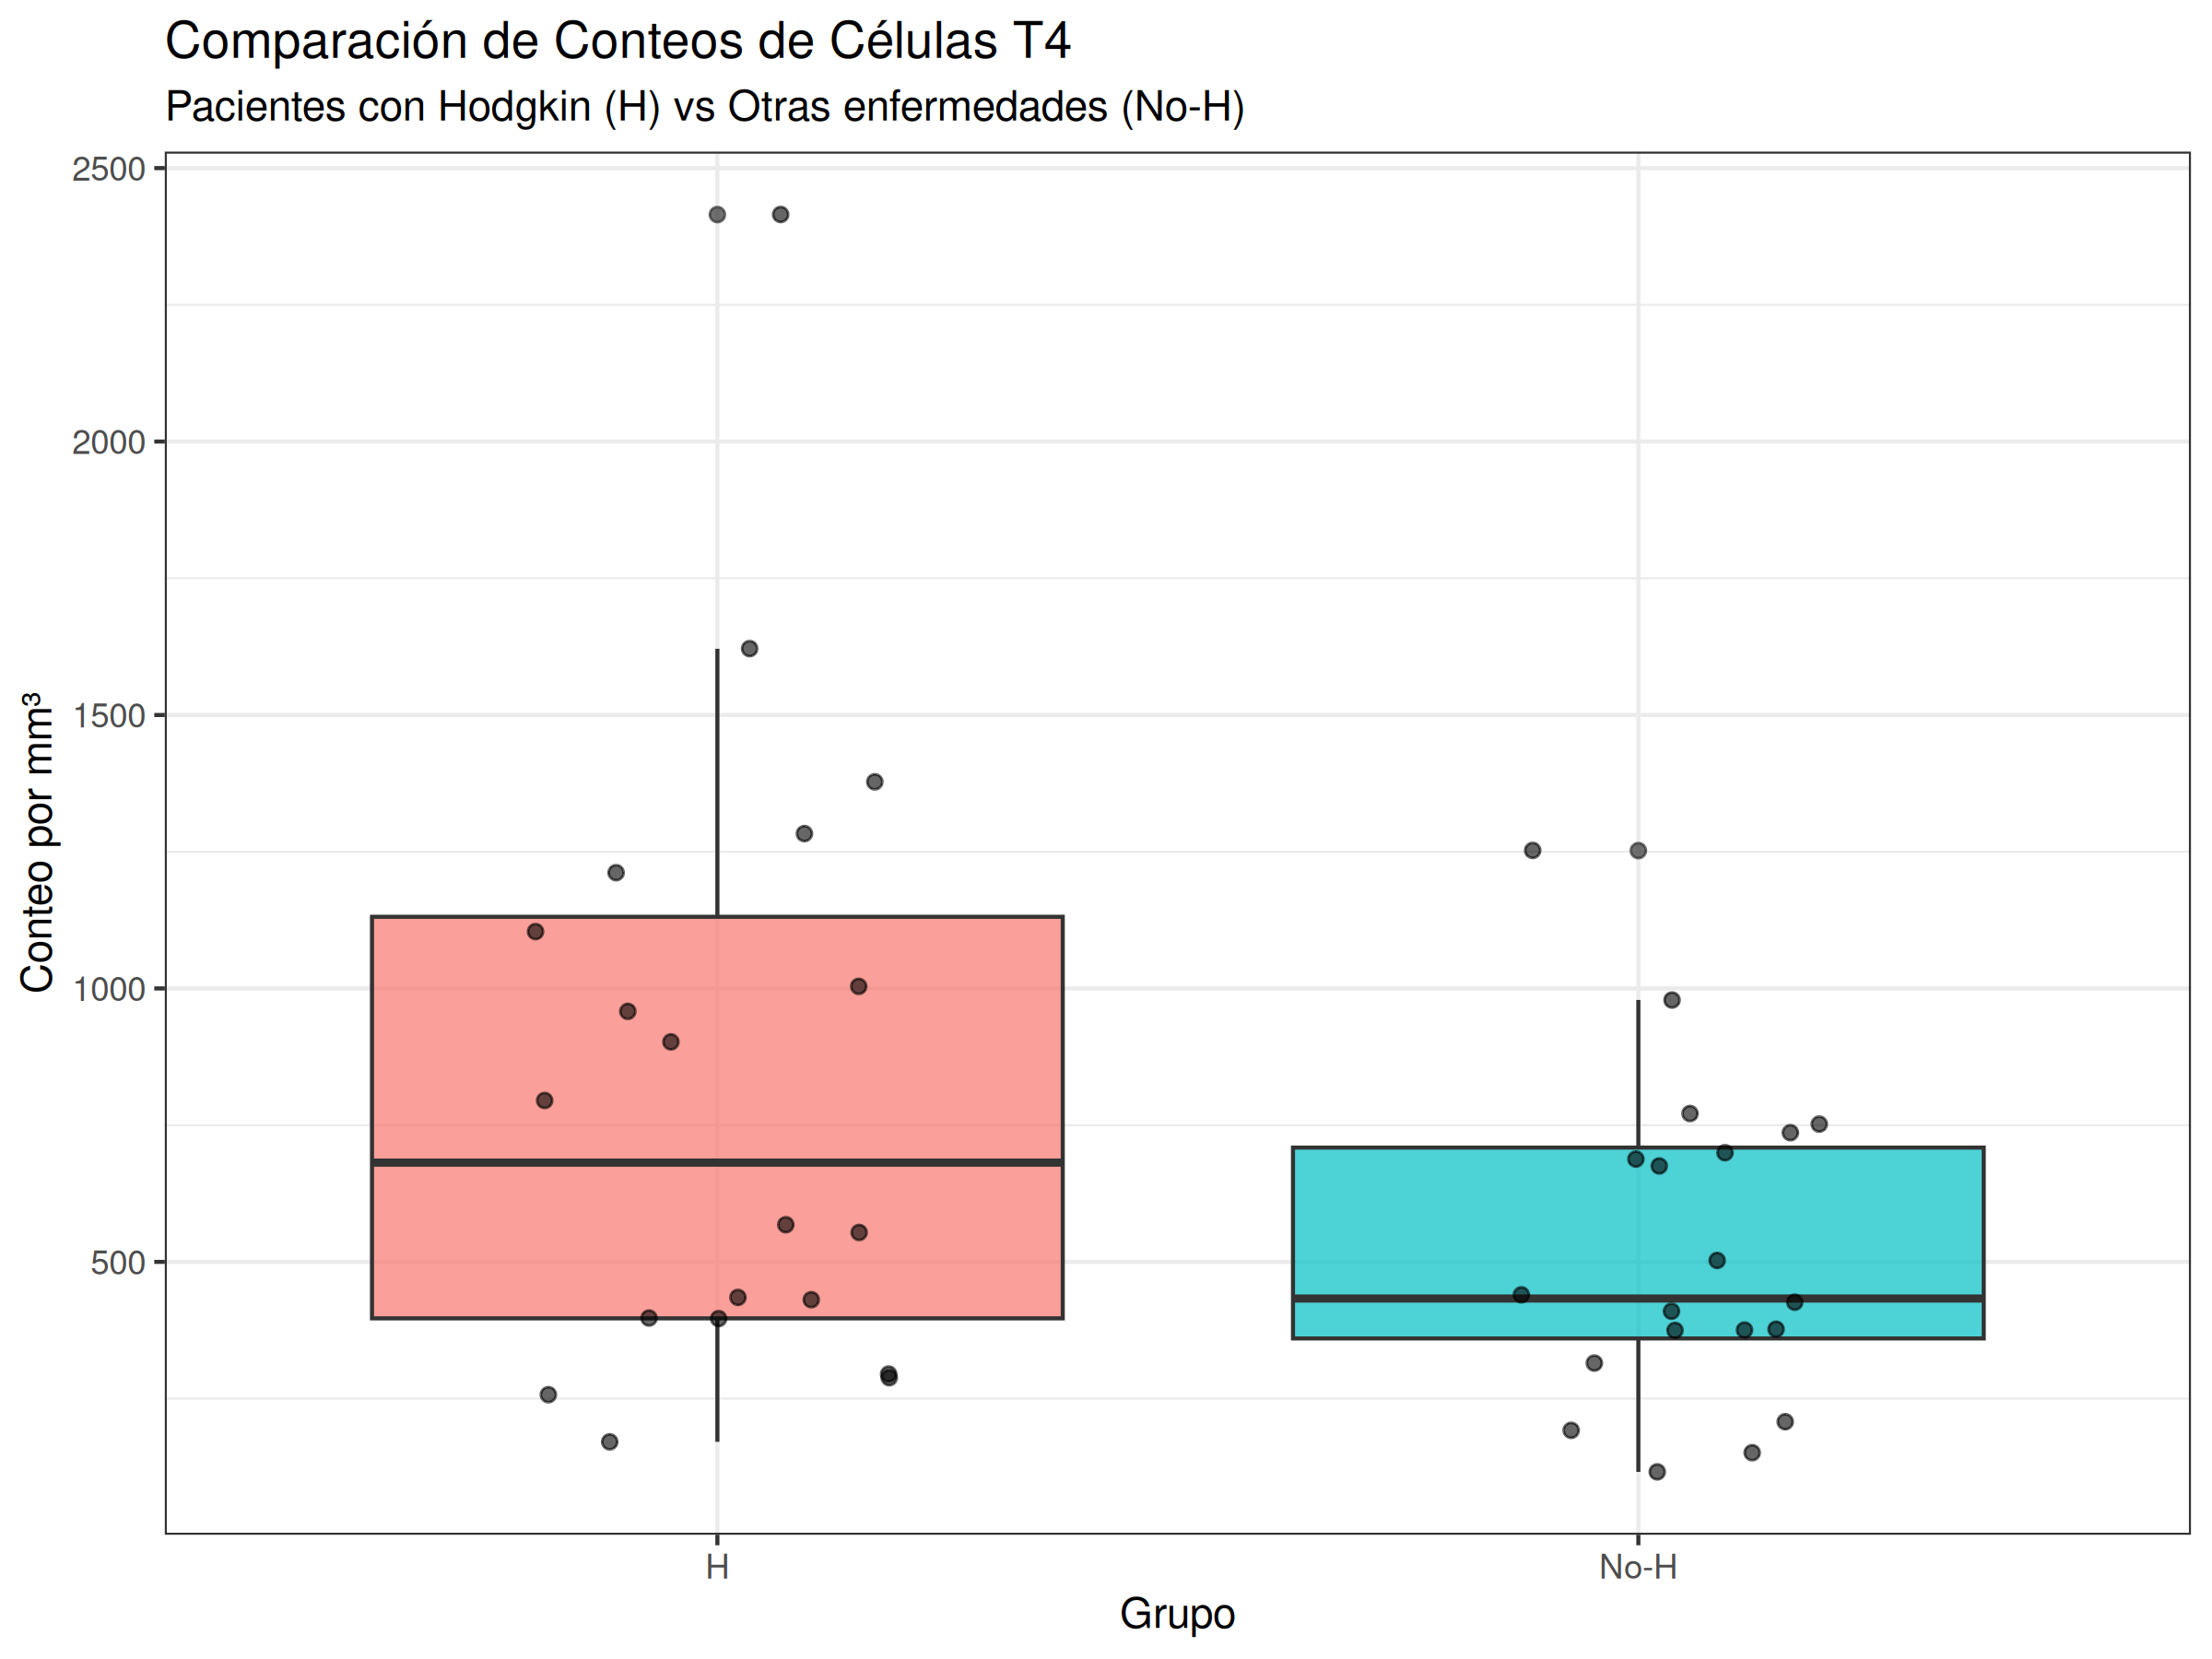
\includegraphics[width=0.6\textwidth]{images/boxplot_comparativo.png}
    \caption{Boxplot de conteos de células T4 para el grupo H y No-H.}
    \label{fig:1}
\end{figure}

En la Figura \ref{fig:1} podemos observar que la mediana del grupo H es mayor en comparación con la del grupo No-H, esto nos sugiere que los pacientes con Hodgkin tienen conteos más altos de células T4 que los otros. También podemos ver que la caja del grupo H es mas grande lo que implica una mayor dispersión de los datos, es decir, mas variabilidad entre el conteo de células T4 de los pacientes mientras que el grupo No-H tiene una caja mas compacta indicando lo opuesto. El grupo H tiene valores muy altos que aparecen como outliers ($\approx$ 2400), el grupo No-H tambien tiene algunos outliers altos pero no tan extremos ($\approx1250$), esto podría indicarnos que la distribución del grupo H podria tener una cola derecha larga. En general el grupo H tiene mayor mediana y mayor dispersión, siendo su distribución más heterogénea y con valores extremos grandes, mientras que el grupo No-H tiene menor mediana, menos dispersión y valores más concentrados.

Para complementar esta descripción visual también se realizaron histogramas de frecuencia:
\begin{figure}[H]
    \centering
    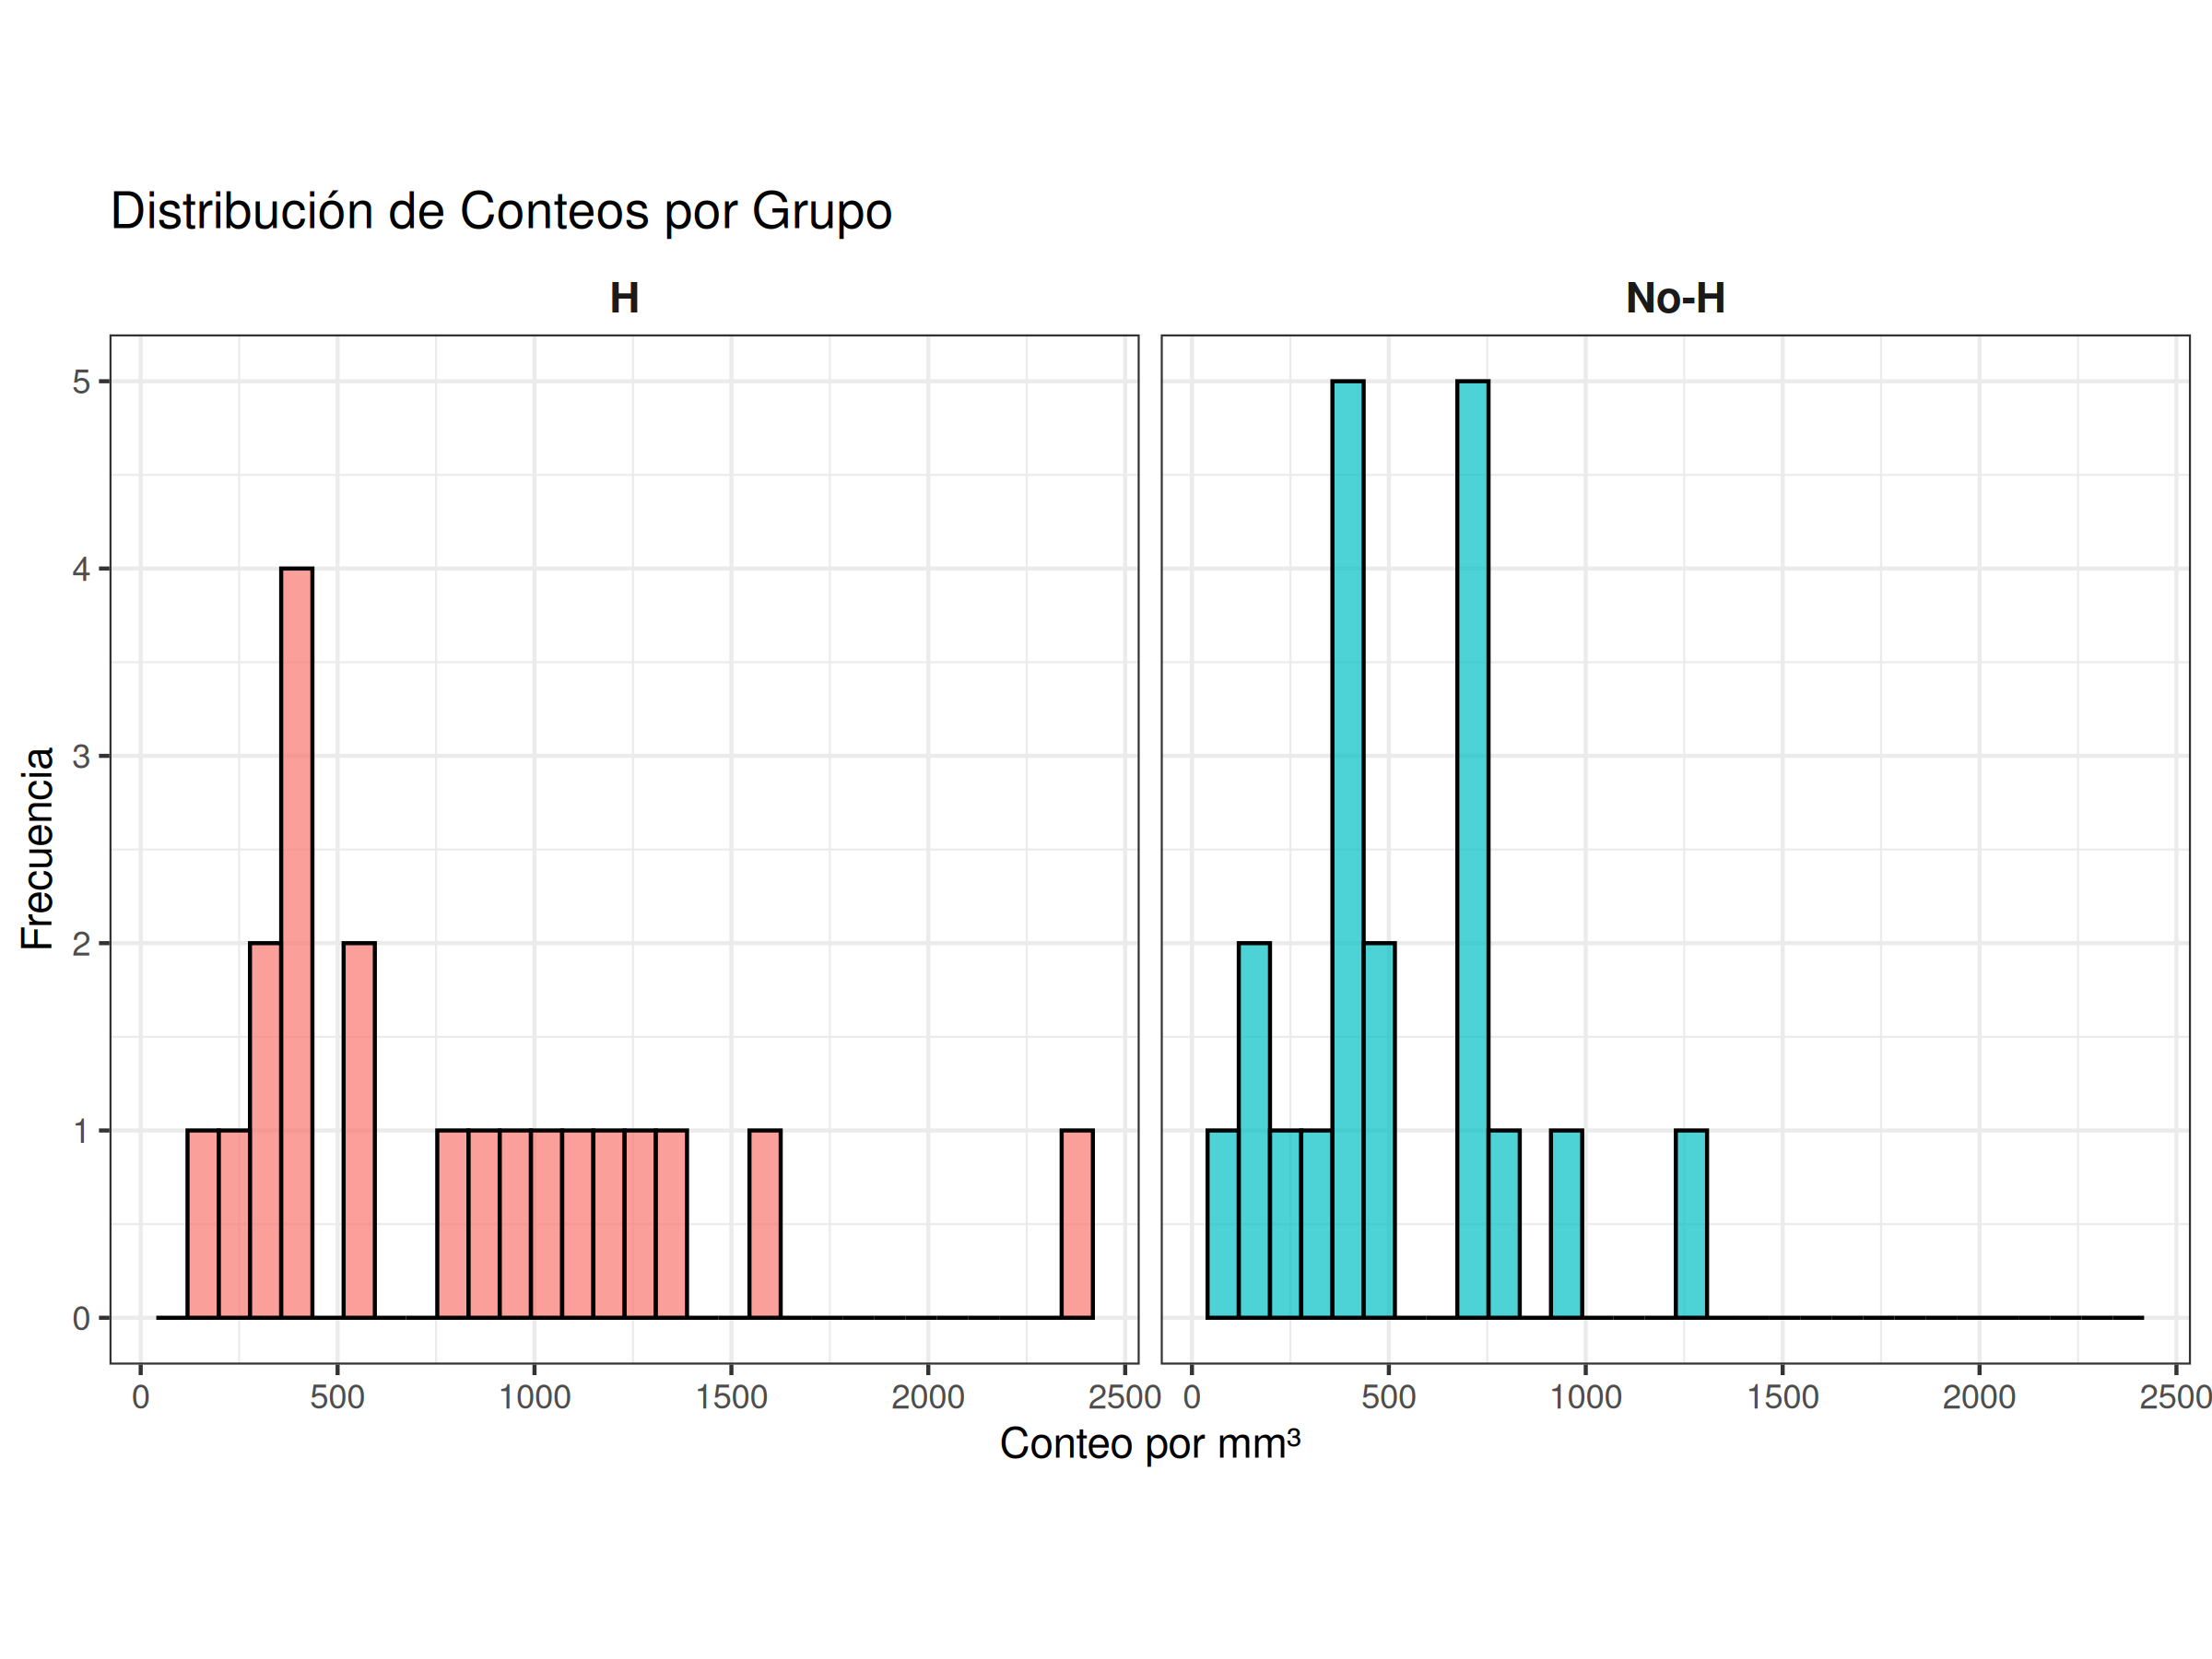
\includegraphics[width=0.7\textwidth]{images/histogramas_comparativos.png}
    \caption{Histogramas de frecuencia de los conteos de células T4 para el grupo H y No-H.}
    \label{fig:2}
\end{figure}

En la Figura \ref{fig:2} podemos observar que la cola larga hacia la derecha que se había sospechado en el boxplot, así mismo podemos ver que los pacientes del grupo H tienden a tener conteos de células T4 mas altos en promedio, mientras que los pacientes del grupo No-H presenta conteos mas bajos y mas consistentes entre si ya que la mayoría de conteos se encuentran agrupados en valores intermedios.

Por ultimo se realizo un gráfico de densidad: 

\begin{figure}[H]
    \centering
    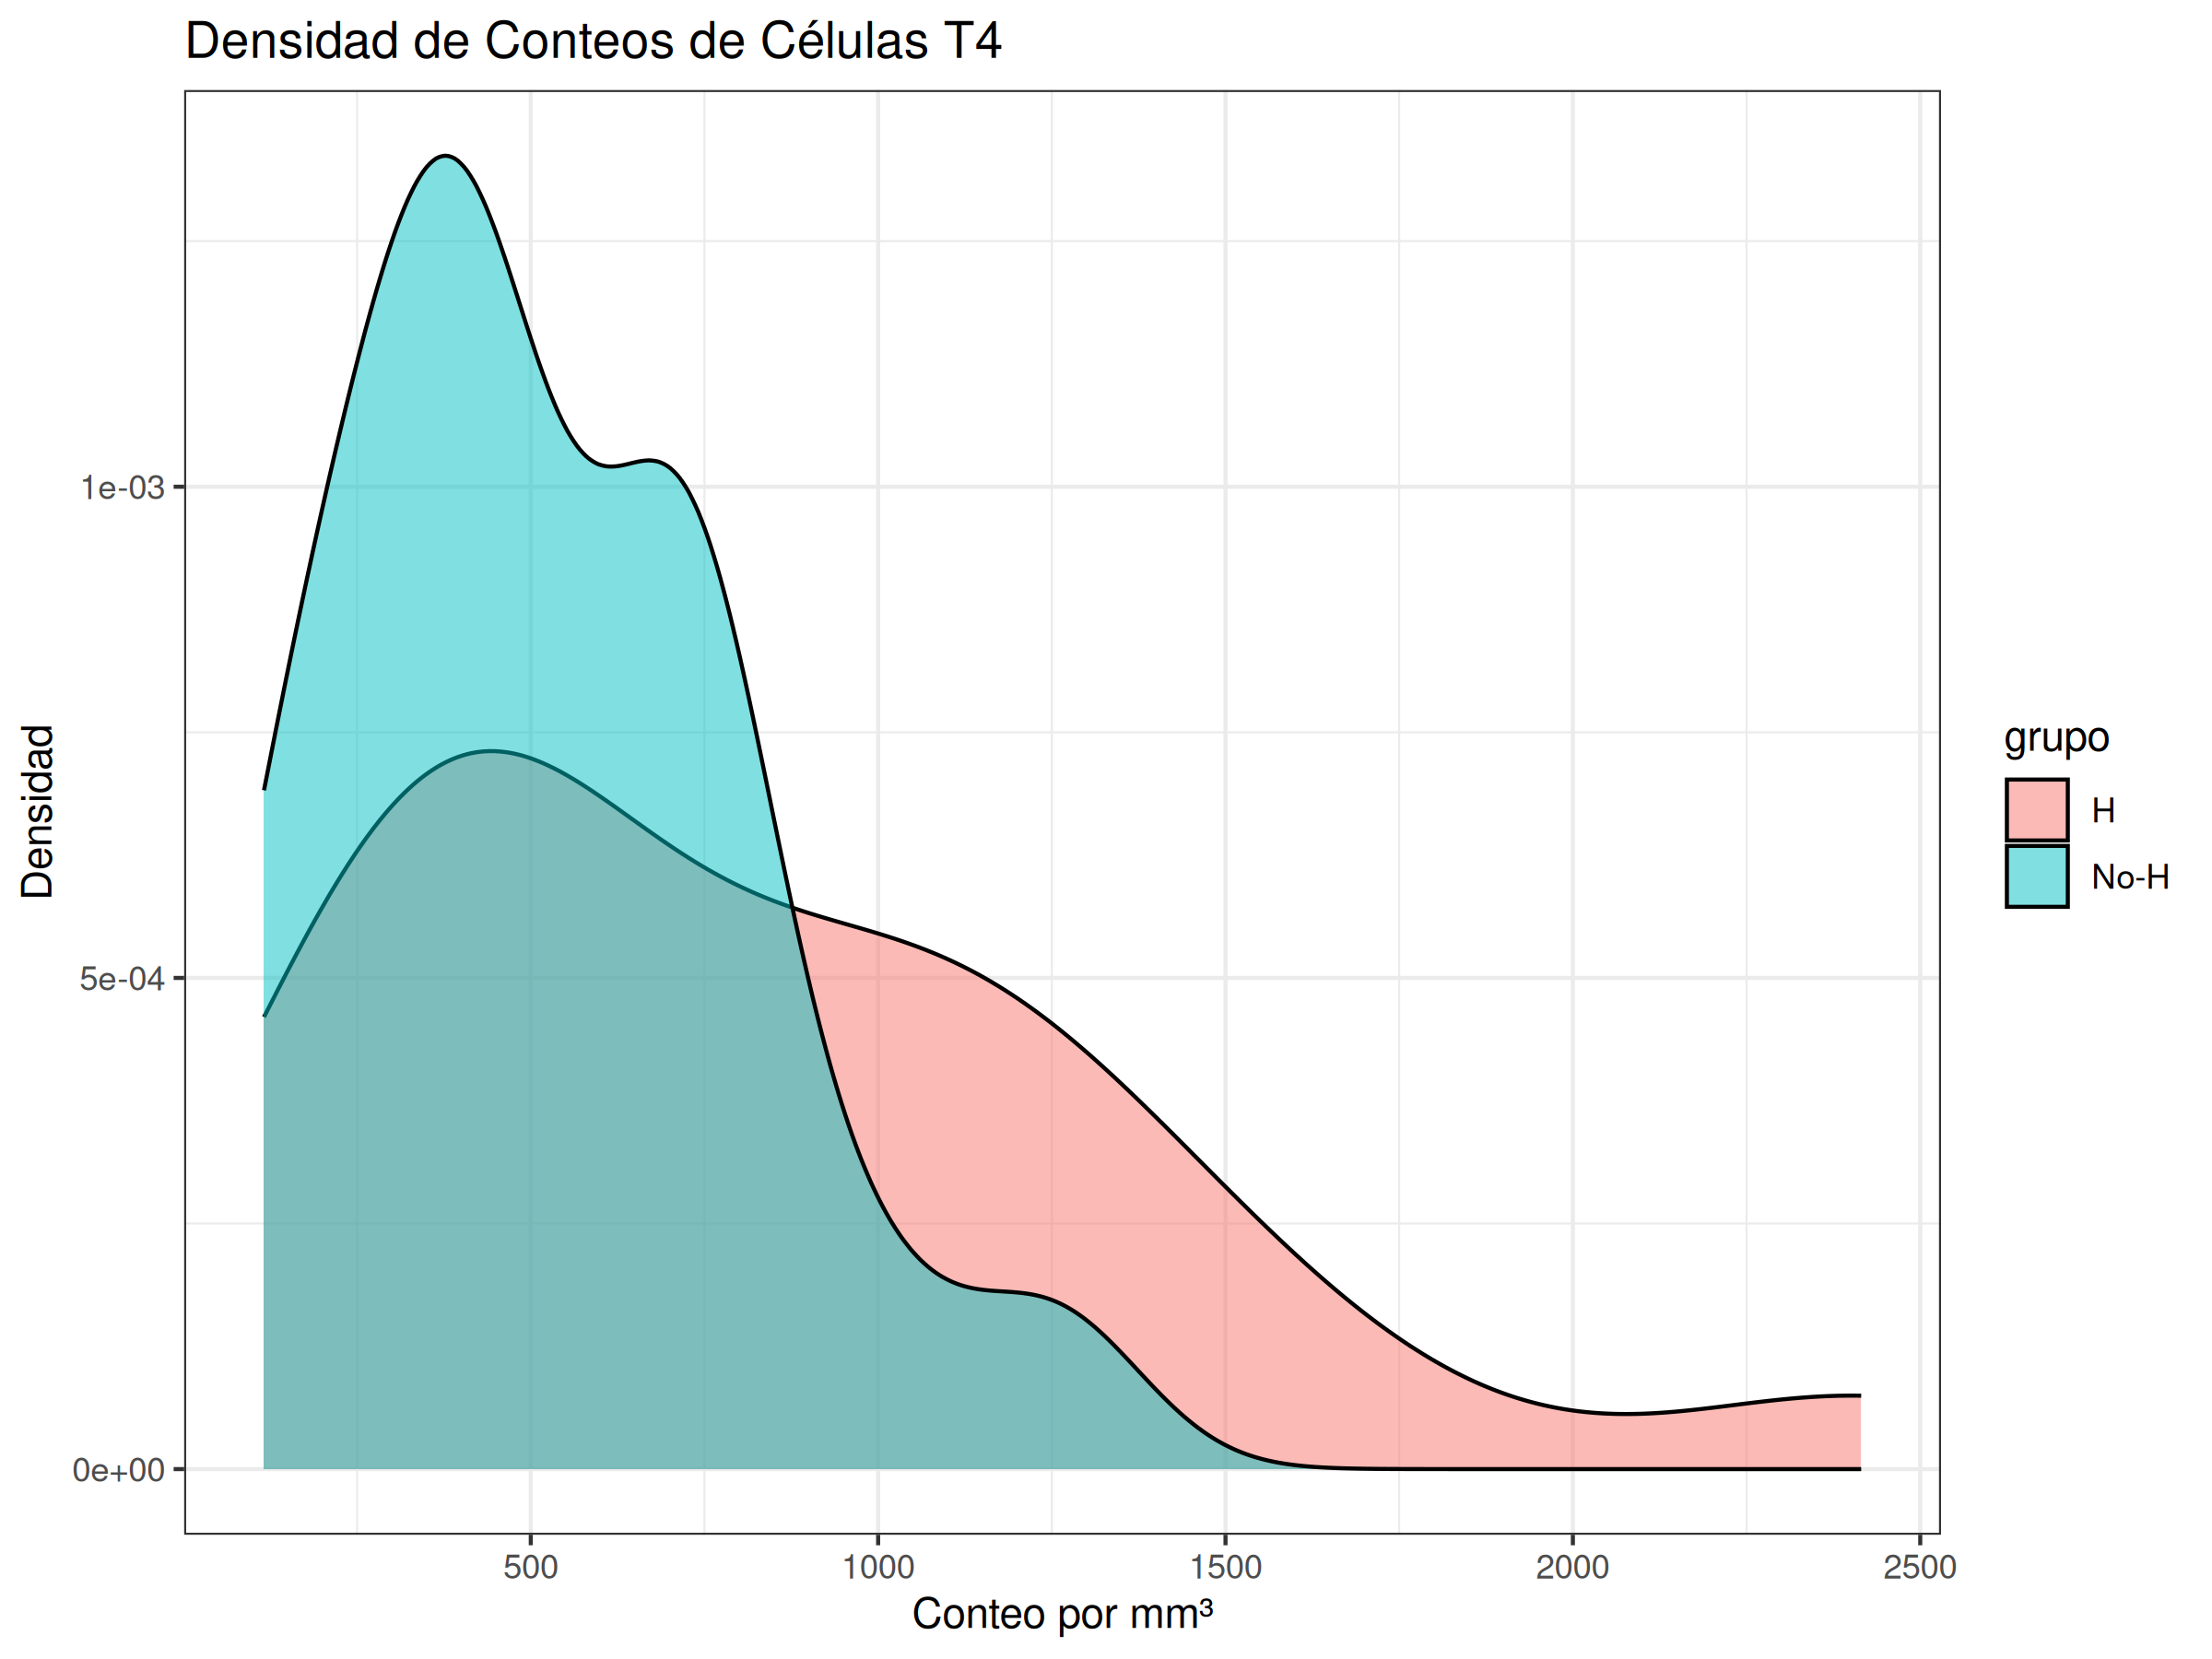
\includegraphics[width=0.55\textwidth]{images/densidad_comparativa.png}
    \caption{Gráfico de densidad de conteos de células T4 para el grupo H y No-H.}
    \label{fig:3}
\end{figure}

La Figura \ref{fig:3} muestra que los conteos de celulas T4 en pacientes del grupo H son más heterogéneos, con una cola derecha larga y valores muy altos, mientras que en pacientes del grupo No-H la distribución es más concentrada en torno a valores moderados y con poca presencia de extremos.

\tcbset{colframe=red, colback=white, boxrule=0.3mm, arc=0mm}
\begin{tcolorbox}
Por lo tanto, en primera instancia estas comparaciones gráficas parecen indicarnos que si existen diferencias en las distribuciones de conteos en ambos grupos.
\end{tcolorbox}

\textbf{b)} En lugar de comparar solo medias con un test clásico, usamos un Modelo Lineal Generalizado (GLM) con respuesta Poisson, que es natural para modelar datos de conteos. Los supuestos del modelo Poisson son los siguientes:

\begin{enumerate}
    \item La variable respuesta $Y_i$ (conteo de células del paciente $i$) sigue una distribución Poisson:
    \begin{equation*}
        Y_i\sim\text{Poisson}(\mu_i), \quad i=1,\dotso,n 
    \end{equation*}
    donde $\mu_i = E(Y_i)$ es la media (también varianza bajo el modelo básico).
    \item Los $Y_i$ son condicionalmente independientes.
    \item La media $\mu_i$ depende de covariables (aquí, el grupo H vs No-H) a través de una función de enlace.
\end{enumerate}

En los GLM con respuesta Poisson, el enlace canónico es el logaritmo:

\begin{equation}
    \log(\mu_i) = \beta_0 + \beta_1 x_i
    \label{eq:3.1}
\end{equation}

Donde:

\begin{itemize}
    \item $x_0 = 0$ si el paciente está en el grupo H,
    \item $x_1 = 1$ si el paciente está en el grupo No-H.
\end{itemize}

Buscamos ajustar este modelo bajo los supuestos mencionados para estimar los parámetros $\beta_0$ y $\beta_1$, siendo cada uno: 

\begin{equation}
    \beta_0 = \log(\mu_\text{H})\quad \text{y} \quad \beta_1 = \log\left(\frac{\mu_{\text{No-H}}}{\mu_\text{H}}\right)
    \label{eq:3.2}
\end{equation}

Entonces, ajustando el modelo mediante la funcion $\texttt{glm()}$ se obtuvo el summary'' siguiente:

\begin{table}[H]
\centering
\caption{Resumen del ajuste del modelo Poisson}
\begin{tabular}{lrrrr}
\hline
 & Estimate & Std. Error & z value & Pr($>|z|$) \\
\hline
Intercept  & 6.713199 & 0.007793 & 861.4 & $<2\times 10^{-16}$$^{***}$ \\
grupoNo-H  & -0.455436 & 0.012511 & -36.4 & $<2\times 10^{-16}$$^{***}$ \\
\hline
\multicolumn{5}{l}{\footnotesize Signif. codes: $^{***}0.001$, $^{**}0.01$, $^{*}0.05$, $^{.}0.1$} \\
\multicolumn{5}{l}{\footnotesize Null deviance: 11325 on 39 d.f.} \\
\multicolumn{5}{l}{\footnotesize Residual deviance: 9965 on 38 d.f.} \\
\multicolumn{5}{l}{\footnotesize AIC: 10294} \\
\multicolumn{5}{l}{\footnotesize Fisher Scoring iterations: 5} \\
\end{tabular}
\end{table}

Podemos observar que el intercepto es $\widehat{\beta}_0 = 6.713$. Esto corresponde al grupo H. Por lo tanto, despejando de la ecuación (\ref{eq:3.2}), tenemos que la media esperada en este grupo es:

\begin{equation*}
    \widehat{\mu}_{\text{H}} = e^{6.713} \approx 824.8
\end{equation*}

Mientras que el efecto del grupo No-H es $\widehat{\beta}_1 = -0.455$. Despejando de la ecuación (\ref{eq:3.2}), esto implica que manteniendo todo lo demás constante, la razón de medias entre No-H y H es:

\begin{equation*}
    \frac{\widehat{\mu}_{\text{No-H}}}{\widehat{\mu}_{\text{H}}} = e^{-0.455} \approx 0.634
\end{equation*}

Es decir, los pacientes No-H presentan, en promedio, un conteo de células T4 aproximadamente un 36.6\% menor que los pacientes del grupo H. 

De acuerdo a los supuestos mencionados, el modelo de Poisson asume que la varianza de $Y_i$ es igual a su media, $\mathrm{Var}(Y_i)=\mu_i$. Sin embargo, en nuestros datos observamos que la desviancia residual ($9965$) es mucho mayor que los grados de libertad residuales ($38$) y que los conteos de T4 muestran gran heterogeneidad y colas largas en el grupo H, lo que sugiere que $\mathrm{Var}(Y_i) \gg E(Y_i)$. Por lo tanto, esto indica una sobre-dispersión, es decir, el modelo Poisson subestima la variabilidad real de los datos.

Para corregir la inferencia, ajustaremos un modelo quasi-Poisson, que conserva la misma forma funcional pero permite que:

\begin{equation*}
    \mathrm{Var}(Y_i) = \phi \, \mu_i
\end{equation*}

donde $\phi > 1$ es un parámetro de dispersión que captura el exceso de variabilidad. De esta manera, los estimadores $\widehat{\beta}$ permanecen iguales, pero sus errores estándar se corrigen multiplicándose por $\sqrt{\phi}$, proporcionando intervalos de confianza y pruebas más realistas.

Ahora, ajustando el modelo quasi-Poisson mediante la función $\texttt{glm()}$ se obtuvo el summary'' siguiente:

\begin{table}[H]
\centering
\caption{Resumen del ajuste del modelo quasi-Poisson}
\begin{tabular}{lrrrr}
\hline
 & Estimate & Std. Error & t value & Pr($>|t|$) \\
\hline
Intercept  & 6.7132 & 0.1297 & 51.750 & $<2\times 10^{-16}$$^{***}$ \\
grupoNo-H  & -0.4554 & 0.2082 & -2.187 & $0.035^{*}$ \\
\hline
\multicolumn{5}{l}{\footnotesize Signif. codes: $^{***}0.001$, $^{**}0.01$, $^{*}0.05$, $^{.}0.1$} \\
\multicolumn{5}{l}{\footnotesize Dispersion parameter: $\phi = 277.0613$} \\
\multicolumn{5}{l}{\footnotesize Null deviance: 11325 on 39 d.f.} \\
\multicolumn{5}{l}{\footnotesize Residual deviance: 9965 on 38 d.f.} \\
\multicolumn{5}{l}{\footnotesize AIC: NA} \\
\multicolumn{5}{l}{\footnotesize Fisher Scoring iterations: 5} \\
\end{tabular}
\end{table}

\tcbset{colframe=red, colback=white, boxrule=0.3mm, arc=0mm}
\begin{tcolorbox}
Podemos ver que tras ajustar por sobredispersión se obtuvo un $\phi = 277.06$ mediante el modelo quasi-Poisson, la diferencia asociada al grupo No-H persistió como estadísticamente significativa con $p = 0.035$.
\end{tcolorbox}

\textbf{c)} Una vez ajustado el modelo quasi-Poisson, que corrige la sobredispersión de los datos, procedemos a evaluar si existe evidencia estadística de una diferencia en las medias de los conteos celulares entre los dos grupos. Para ello, utilizamos la normalidad asintótica de los estimadores de máxima verosimilitud para construir un intervalo de confianza para el parámetro $\beta_1$, que representa el efecto del grupo No-H en la escala logarítmica. Del resumen del modelo quasi-Poisson, obtuvimos que $\widehat{\beta}_1= -0.4554$ y un error estándar: 0.2082.

Para construir un intervalo de confianza del 90\%, usamos el valor crítico correspondiente a un nivel de significancia de $\alpha=0.10$, es decir, $z_{0.95}\approx1.645$ proveniente de una distribución normal estándar. 

\newpage
El intervalo se calcula como:

\begin{align*}
\widehat{\beta}_1 \pm z_{0.95} \cdot SE(\hat{\beta}_1) &= -0.4554 \pm 1.645 \cdot 0.2082 \\
&= -0.4554 \pm 0.3425 \\
&= [-0.7979, -0.1129]
\end{align*}

El intervalo de confianza del 90\% para $\beta_1$ es [-0.798, -0.113]. Dado que este intervalo está completamente por debajo de cero y no lo incluye, existe evidencia estadística significativa (con un nivel de confianza del 90\%) de que la media de conteos en el grupo No-H es diferente a la del grupo H.

Para facilitar la interpretación, podemos transformar este resultado a la escala original (razón de medias) exponenciando los límites del intervalo:

\begin{equation*}
    IC_{90\%}\left(\frac{\mu_{\text{No-H}}}{\mu_{\text{H}}}\right) = [e^{-0.7979}, e^{-0.1129}] \approx [0.450, 0.893]
\end{equation*}

\begin{center}
\fcolorbox{red}{white}{$\displaystyle\Rightarrow IC_{90\%}\left(\frac{\mu_{\text{No-H}}}{\mu_{\text{H}}}\right) \approx [0.450, 0.893]$}
\end{center}

Este intervalo para la razón de medias no contiene el valor 1, lo que confirma nuestra conclusión. Específicamente, podemos afirmar con un 90\% de confianza que la media de conteos de células T4 en los pacientes del grupo No-H es entre un 45\% y un 89.3\% de la media de los pacientes del grupo H. 

\tcbset{colframe=red, colback=white, boxrule=0.3mm, arc=0mm}
\begin{tcolorbox}
Por lo tanto, los pacientes del grupo No-H tienen, en promedio, un conteo celular significativamente menor.
\end{tcolorbox}


\newpage

\appendix  
\section{Código en \textcolor{CIMATRed}{R}}

A continuación, se presentan los scripts de \texttt{R} utilizados para la carga de datos, el análisis exploratorio y el ajuste de los modelos estadísticos discutidos en este reporte.

% --- Script 1 ---
\begin{lstlisting}[language=R, caption={Script 1: Carga y Limpieza de Datos - Conteos de Células T4.}, label={lst:script1}]
# =============================================================================
# Script 1: Carga y Limpieza de Datos - Conteos de Celulas T4
# Autor: Diego Paniagua Molina
# Fecha: 2025-08-29
# =============================================================================

# Instalar paquetes necesarios ------------------------------------------------
if (!require("dplyr")) install.packages("dplyr")
if (!require("readr")) install.packages("readr")
if (!require("here")) install.packages("here")

# Cargar paquetes -------------------------------------------------------------
library(dplyr)
library(readr)
library(here)

# Crear los datos manualmente -------------------------------------------------
datos <- tibble(
  grupo = rep(c("H", "No-H"), each = 20),
  conteo = c(
    # Grupo H (Hodgkin) - Primera fila
    396, 568, 1212, 171, 554, 1104, 257, 435, 295, 397,
    # Grupo H (Hodgkin) - Segunda fila  
    288, 1004, 431, 795, 1621, 1378, 902, 958, 1283, 2415,
    # Grupo No-H (No Hodgkin) - Primera fila
    375, 375, 752, 208, 151, 116, 736, 192, 315, 1252,
    # Grupo No-H (No Hodgkin) - Segunda fila
    675, 700, 440, 771, 688, 426, 410, 979, 377, 503
  )
)

# Verificar estructura de los datos -------------------------------------------
cat("Estructura de los datos:\n")
glimpse(datos)

cat("\nResumen por grupos:\n")
datos %>%
  group_by(grupo) %>%
  summarise(
    n = n(),
    media = mean(conteo),
    mediana = median(conteo),
    sd = sd(conteo),
    min = min(conteo),
    max = max(conteo)
  ) %>%
  print()

# Guardar datos en formato CSV ------------------------------------------------
dir.create(here("data"), recursive = TRUE, showWarnings = FALSE)
write_csv(datos, here("data", "raw", "datos_pacientes.csv"))

# Mensaje de confirmacion -----------------------------------------------------
cat("\nDatos creados y guardados en: data/raw/datos_pacientes.csv\n")
cat("Total de observaciones:", nrow(datos), "\n")
cat("Grupos:", unique(datos$grupo), "\n")
\end{lstlisting}

\clearpage % Inicia el segundo script en una nueva página

% --- Script 2 ---
\begin{lstlisting}[language=R, caption={Script 2: Analisis Exploratorio - Comparacion Grafica (Inciso a).}, label={lst:script2}]
# =============================================================================
# Script 2: Analisis Exploratorio - Comparacion Grafica (Inciso a)
# =============================================================================

# Instalar paquetes necesarios ------------------------------------------------
if (!require("dplyr")) install.packages("dplyr")
if (!require("ggplot2")) install.packages("ggplot2")
if (!require("here")) install.packages("here")

# Cargar paquetes -------------------------------------------------------------
library(dplyr)
library(ggplot2)
library(here)

# Cargar datos ----------------------------------------------------------------
datos <- read_csv(here("data", "raw", "datos_pacientes.csv"), show_col_types = FALSE)

# 1. Boxplot comparativo con puntos -------------------------------------------
boxplot <- ggplot(datos, aes(x = grupo, y = conteo, fill = grupo)) +
  geom_boxplot(alpha = 0.7) +
  geom_point(position = position_jitter(width = 0.2), alpha = 0.6) +
  labs(title = "Comparacion de Conteos de Celulas T4",
       subtitle = "Pacientes con Hodgkin (H) vs Otras enfermedades (No-H)",
       x = "Grupo",
       y = "Conteo por mm³") +
  theme_bw() +
  theme(legend.position = "none")

# 2. Histogramas comparativos -------------------------------------------------
histogramas <- ggplot(datos, aes(x = conteo, fill = grupo)) +
  geom_histogram(alpha = 0.7, position = "identity", color = "black") +
  facet_wrap(~ grupo, nrow = 1) +  
  labs(title = "Distribucion de Conteos por Grupo",
       x = "Conteo por mm³",
       y = "Frecuencia") +
  theme_bw() +
  theme(aspect.ratio = 1,
        legend.position = "none",
        strip.background = element_blank(),  
        strip.text = element_text(face = "bold", size = 11)) 

# 3. Grafico de densidad ------------------------------------------------------
densidad <- ggplot(datos, aes(x = conteo, fill = grupo)) +
  geom_density(alpha = 0.5) +
  labs(title = "Densidad de Conteos de Celulas T4",
       x = "Conteo por mm³",
       y = "Densidad") +
  theme_bw()

# Guardar graficos ------------------------------------------------------------
dir.create(here("results", "figures"), recursive = TRUE, showWarnings = FALSE)
ggsave(here("results", "figures", "boxplot_comparativo.png"), 
       plot = boxplot, width = 8, height = 6, dpi = 300)
ggsave(here("results", "figures", "histogramas_comparativos.png"), 
       plot = histogramas, width = 8, height = 6, dpi = 300)
ggsave(here("results", "figures", "densidad_comparativa.png"), 
       plot = densidad, width = 8, height = 6, dpi = 300)

# Mostrar graficos ------------------------------------------------------------
print(boxplot)
print(histogramas)
print(densidad)

cat("\n Graficos guardados en la carpeta: results/figures/\n")
\end{lstlisting}

\clearpage % Inicia el tercer script en una nueva página

% --- Script 3 ---
\begin{lstlisting}[language=R, caption={Script 3: Modelo de Poisson e Inferencia (Inciso b).}, label={lst:script3}]
# =============================================================================
# Script 3: Modelo de Poisson e Inferencia (Inciso b)
# =============================================================================

# Instalar paquetes necesarios ------------------------------------------------
if (!require("dplyr")) install.packages("dplyr")
if (!require("readr")) install.packages("readr")
if (!require("here")) install.packages("here")

# Cargar paquetes -------------------------------------------------------------
library(dplyr)
library(readr)
library(here)

# Cargar datos ----------------------------------------------------------------
datos <- read_csv(here("data", "raw", "datos_pacientes.csv"), show_col_types = FALSE)

# INCISO b: Ajustar modelo de Poisson -----------------------------------------
cat("Ajustando modelo de Poisson...\n")

# Modelo: log(conteo) = beta_0 + beta_1*grupo
modelo_poisson <- glm(conteo ~ grupo, 
                      family = poisson(link = "log"),
                      data = datos)

# Resumen del modelo ----------------------------------------------------------
cat("\nResumen del modelo de Poisson:\n")
resumen_modelo <- summary(modelo_poisson)
print(resumen_modelo)

# Verificar sobredispersion ---------------------------------------------------
cat("\nVerificacion de sobredispersion:\n")
deviance_val <- resumen_modelo$deviance
df_residual <- resumen_modelo$df.residual
ratio_sobredispersion <- deviance_val / df_residual

cat("Deviance:", deviance_val, "\n")
cat("Grados de libertad:", df_residual, "\n")
cat("Ratio Deviance/df:", ratio_sobredispersion, "\n")

# Guardar modelo --------------------------------------------------------------
dir.create(here("results", "models"), recursive = TRUE, showWarnings = FALSE)
saveRDS(modelo_poisson, here("results", "models", "modelo_poisson.rds"))
cat("\n Modelo guardado en: results/models/modelo_poisson.rds\n")

# Existe sobredispersion, ajustar modelo quasi-Poisson ------------------------
cat("\nAjustando modelo quasi-Poisson...\n")

modelo_quasi <- glm(conteo ~ grupo,
                    family = quasipoisson(link = "log"),
                    data = datos)

# Resumen del modelo ---------------------------------------------------------- 
cat("\nResumen del modelo quasi-Poisson:\n")
resumen_quasi <- summary(modelo_quasi)
print(resumen_quasi)

# Dispersion (phi) ------------------------------------------------------------
phi <- resumen_quasi$dispersion
cat("\nEstimador de dispersion (phi):", round(phi, 3), "\n")

# Guardar modelo --------------------------------------------------------------
saveRDS(modelo_quasi, here("results", "models", "modelo_quasipoisson.rds"))
cat("\n Modelo guardado en: results/models/modelo_quasipoisson.rds\n")
\end{lstlisting}